\documentclass[tikz, border=2pt]{standalone}

\usepackage{amsmath,amssymb}
\usepackage{pgfplots}
\pgfplotsset{compat=1.18}
\usepackage{xcolor}

\definecolor{utnblue}{RGB}{0, 51, 102}
\definecolor{utnred}{RGB}{204, 0, 0}
\definecolor{utngreen}{RGB}{0, 130, 70}

\begin{document}
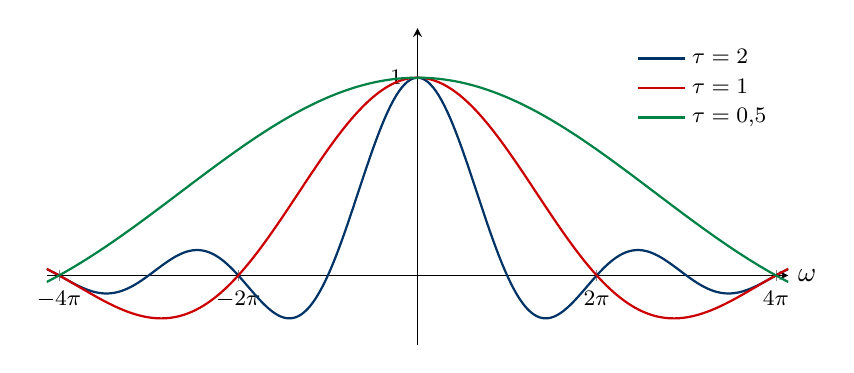
\begin{tikzpicture}
\begin{axis}[
    width=11cm, height=5.6cm,
    axis lines=middle,
    enlargelimits=false,
    tick label style={font=\footnotesize},
    label style={font=\small},
    xlabel={$\omega$},
    every axis x label/.style={at={(ticklabel* cs:1)}, anchor=west},
    xmin=-13, xmax=13, ymin=-0.35, ymax=1.25,
    xtick={-12.566,-6.2832,6.2832,12.566},
    xticklabels={$-4\pi$,$-2\pi$,$2\pi$,$4\pi$},
    ytick={1}, yticklabels={$1$},
    legend style={font=\footnotesize, draw=none, at={(0.99,0.97)}, anchor=north east},
    legend cell align=left,
]
% tau = 2 : sinc(w)
\addplot[utnblue, thick, samples=260, domain=-13:13] {sin(deg(x))/x};
\addlegendentry{$\tau=2$}
% tau = 1 : sinc(w/2)
\addplot[utnred, thick, samples=260, domain=-13:13] {sin(deg(x/2))/(x/2)};
\addlegendentry{$\tau=1$}
% tau = 0.5 : sinc(w/4)
\addplot[utngreen, thick, samples=260, domain=-13:13] {sin(deg(x/4))/(x/4)};
\addlegendentry{$\tau=0{,}5$}
\end{axis}
\end{tikzpicture}
\end{document}
